\documentclass{VUMIFPSkursinis}
\usepackage{algorithmicx}
\usepackage{algorithm}
\usepackage{algpseudocode}
\usepackage{amsfonts}
\usepackage{amsmath}
\usepackage{bm}
\usepackage{caption}
\usepackage{color}
\usepackage{float}
\usepackage{graphicx}
\usepackage{listings}
\usepackage{subfig}
\usepackage{wrapfig}
\usepackage{enumitem}
\usepackage{makecell}
\usepackage{hyperref}
% \usepackage{slashbox}

% Titulinio aprašas
\university{Vilniaus universitetas}
\faculty{Matematikos ir informatikos fakultetas}
\department{Programų sistemų studijų programa}
\papertype{Kursinis darbas}
\title{Likvidavimo algoritmo tobulinimas perviršinio užstato skolinimo protokoluose}
\titleineng{Improving liquidation algorithms in over-collateralized lending protocols}
\status{4 kurso 4 grupės studentas}
\author{Vismantas Stonkus}
\supervisor{Prof. dr. Remigijus Paulavičius}
\date{Vilnius – \the\year}

% Nustatymai
% \setmainfont{Palemonas}   % Pakeisti teksto šriftą į Palemonas (turi būti įdiegtas sistemoje)
\bibliography{bibliografija}

\begin{document}
\maketitle

\tableofcontents

\sectionnonum{Įvadas}

Kriptovaliutos, kaip sparčiai auganti finansinė sritis, yra populiarus objektas spekuliantams, kurie siekia pasipelnyti iš šių valiutų vertės svyravimų. Nepaisant didelių pelningumo galimybių, investavimas į kriptovaliutas neatsiejamas nuo rizikos, kad valiutos vertė gali smarkiai nukristi, dėl ko investuotojas gali prarasti dalį ar net visą pradinę investiciją. Siekiant maksimalaus pelno ir minimalios rizikos yra taikomi automatiniai arbitražo algoritmai. Šie algoritmai analizuoja kriptovaliutų rinkos svyravimus ir automatiškai vykdo sandorius, leidžiančius pasipelnyti iš mažiausių kainų skirtumų tarp skirtingų biržų.

Šiame darbe dėmesys yra sutelktas į likvidacijos procesą ir jo integravimą į esamus automatinio arbitražo algoritmus. Darbo tikslas – analizuoti ir palyginti skirtingas likvidavimo strategijas perviršinio užstato skolinimo protokoluose, siekiant sukurti ir optimizuoti algoritmą, kuris maksimaliai padidintų likvidatoriaus pelną, efektyviai išnaudojant rinkos svyravimus ir automatizuoto arbitražo galimybes.

Tam, kad darbo tikslas būtų įgyvendintas buvo išsikelti uždaviniai:
\begin{enumerate}
    \item Apžvelgti esamus perviršinio užstato skolinimo protokolus bei jų veikimo principus.
    \item Išnagrinėti likvidavimo proceso mechanizmą.
    \item Sukurti ar pamodifikuoti algoritmą, skirtą efektyviam likvidavimo strategijų vykdymui automatizuoto arbitražo sąlygomis.
    \item Palyginti sukurtą algoritmą su egzistuojančiais sprendimais, įvertinant pelningumą.
\end{enumerate}

Darbo struktūra yra sudaryta iš kelių pagrindinių skyrių. Pirmajame skyriuje pristatoma, kas yra arbitražas, siekiant suteikti teorinį pagrindą. Antrajame skyriuje aptariamos likvidacijos, jų svarba ir galimybės kriptovaliutų pasaulyje. Trečiajame skyriuje analizuojamos skirtingos likvidacijų strategijos, o ketvirtajame skyriuje pateikiami tyrimo rezultatai, įskaitant pelningumo skaičiavimus, strategijų realizacijos pavyzdžius ir duomenų analizę. Darbas užbaigiamas rezultatais ir išvadomis, kurios apibendrina pagrindines darbo įžvalgas.

\section{Kas yra arbitražas}
Arbitražas yra finansinė strategija, grindžiama ekonominių skirtumų išnaudojimu tarp dviejų ar daugiau rinkų, siekiant gauti pelną be jokios rizikos ar su minimalia rizika. Paprastai tariant, tai yra praktika, kai investuotojai perka tam tikrus finansinius instrumentus, tokius kaip prekės ar valiutos pigesnėje rinkoje, ir tuoj pat pardavinėja juos brangesnėje rinkoje, gaudami pelną iš šio kainų skirtumo.

Vienas esminių arbitražo principų yra reliatyvumas -- investuotojai renkasi referencinę valiutą, kurios vertę jie laiko stabilia ir dirba siekdami padidinti šios valiutos kiekį. Pavyzdžiui, jei arbitražininkas laiko eurą stabilia valiuta, jis perka ir parduoda kitas valiutas arba kitokį turtą, tikėdamasis gauti kuo didesnį pelną eurais.

Paprasčiausias arbitražas susideda iš kainų skirtumų tarp dviejų rinkų. Tai pasiekiama konvertuojant stabilų turto vienetą į kitą valiutą pagal kursą $P_1$ ir vėliau konvertuojant šią valiutą atgal į pradinį stabilų turto vienetą kursu $P_2$, kur $P_1 \cdot P_2 > 1$. Šią pagrindinę idėją galima plėtoti ir modifikuoti įvairiais būdais:

\begin{itemize}
    \item įtraukti tarpinius konvertavimo žingsnius, sudarant ilgesnę operacijų grandinę, siekiant išnaudoti kainų skirtumus biržose, kuriose nėra tiesioginio konvertavimo kelio iš ar į stabiliąją valiutą;
    \item pradėti arbitražą ne vien tik su viena stabiliąja valiuta, bet su keliomis. Taip galima efektyviau išnaudoti turimą kapitalą, nes skirtingos stabilių valiutų pozicijos gali suteikti daugiau lankstumo ir galimybių reaguoti į kainų skirtumus įvairiose biržose;
    \item išskaidyti valiutos konvertavimą į kitą per kelias biržas, siekiant išvengti didelio kainų svyravimo vienoje biržoje;
    \item konvertuoti vieną turto vienetą į kelias skirtingas valiutas vienoje tranzakcijoje dėl tam tikrų platformų galimybių;
    \item pasiskolinti kapitalą iš biržos su sąlyga, kad skola bus grąžinta per arbitražo procesą, taip panaikinant reikalavimą turėti pradinį kapitalą.
\end{itemize}

Efektyviausia arbitražo ypatumus pateikti pasinaudojant grafais. Pavyzdžiui, grafe, kur mazgai reprezentuoja savininkų sąskaitas (tradicinių valiutų atveju) arba piniginės adresus (kriptovaliutų atveju), o kryptinės briaunos – valiutų ar kriptovaliutų persiuntimus tarp jų, aiškiai matoma turtų judėjimo dinamika ir galimos arbitražo pelno galimybės. 

\begin{figure}[H]
    \centering
    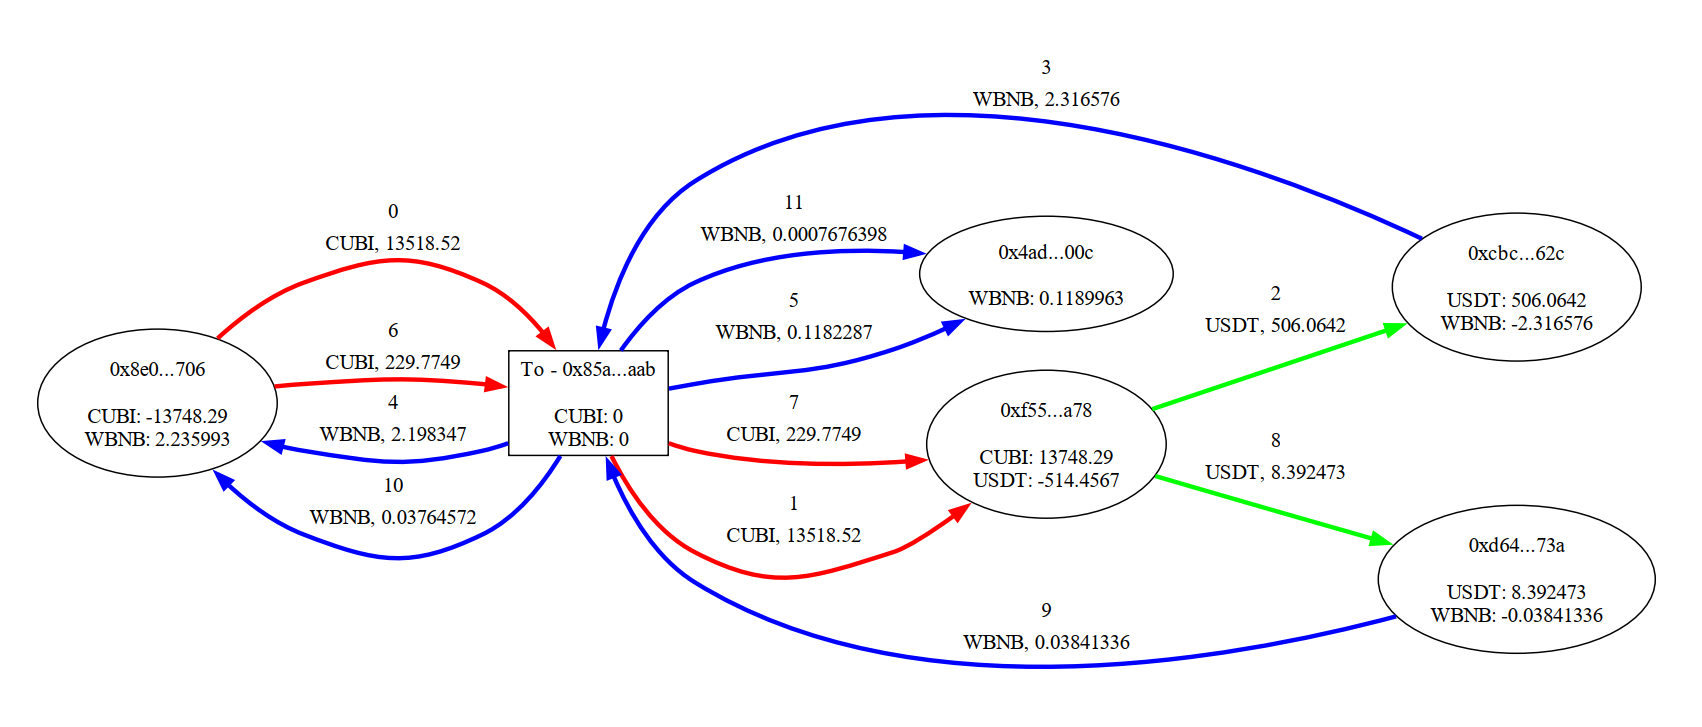
\includegraphics[scale=0.3]{img/arb1.png}
    \caption{Arbitražo vizualizacija: lėšų pervedimai ir galutinis pelnas – 0,11899 WBNB}
    \label{img:chess-minimax-2}
\end{figure} 

\ref{img:chess-minimax-2} pav. pateikta arbitražo vizualizacija kriptovaliutų atveju. Matome 12 pavedimų tarp skirtingų piniginių adresų (numeracija prasideda nuo 0). Šiuo atveju adresas 0x85a..aab yra pradinis kontrakto adresas, kuris buvo iškviestas tranzakcijoje. Iš viso tranzakcijoje dalyvauja 4 rinkos, kuriose galima konvertuoti valiutų poras:

\begin{itemize}
    \item 0x8eo..706 -- CUBI - WBNB
    \item 0xf55..a78 -- CUBI - USDT
    \item 0xcbc..62c -- USDT - WBNB
    \item 0xd64..73a -- USDT - WBNB
\end{itemize}

Adresas 0x4ad..00c šiuo atveju yra tik pelno piniginė, kurioje tranzakcijos pabaigoje atsiranda papildomi 0,11899 WBNB valiutos.

Kiekviename mazge taip pat pažymėtos valiutos ir jų kiekiai, nurodantys galutinį valiutos skirtumą po tranzakcijos. Pavyzdžiui, rinkoje 0x8eo..706 valiuta WBNB -> CUBI buvo konvertuota du kartus, kur iš viso į rinką įdėta 2,235993 WBNB, o išimta 13748,29 CUBI.

Tranzakciją galima suskirstyti į dvi dalis su pavedimais 0-5 ir 6-11. Pirmuosiuose penkiuose pavedimuose (0-4) atliekamas ratas: pradžioje trumpam pasiskolinama CUBI, tada ji iškeičiama į USDT, o po to -- į WBNB. Trečiuoju pavedimu gaunama daugiau valiutos, nei reikia skolai grąžinti ketvirtuoju pavedimu. Todėl perviršis lieka kaip pelnas, kuris penktuoju pavedimu persiunčiamas į pelno piniginę. Panašiai vyksta ir su pavedimais 6-11, tačiau antrojoje dalyje naudojama kita USDT-WBNB rinka, o apskritai keičiamų valiutos kiekių dydžiai yra mažesni.

\section{Likvidacijos}

\subsection{Paskolų platformos}
Paskolų platformos – tai sistemos, kuriose vartotojai gali skolintis ar skolinti pinigus kitiems vartotojams. Tradicinėse bankinėse sistemose bankas veikia kaip tarpininkas tarp skolintojo ir skolininko. Paskolų platformose šis tarpininkavimo procesas dažnai yra automatizuotas.

\subsubsection{Veiklos principas}
\begin{itemize}
    \item \textbf{Skolintojai}: asmenys ar įmonės, turintys perteklinių lėšų, kurias jie norėtų investuoti, kad gautų grąžą kaip palūkanas.
    \item \textbf{Skolininkai}: asmenys ar įmonės, kuriems reikia lėšų įvairiems tikslams – pradėti verslą, finansuoti projektą, pirkti prekę ir pan.
\end{itemize}

Skolintojai įneša savo lėšas į platformą, o skolininkai pateikia prašymus dėl paskolų. Platforma tada suderina šiuos du suinteresuotus šalių poreikius. Priklausomai nuo platformos ir paskolos tipo, gali būti reikalaujama, kad skolininkai užstatytų tam tikrą turto dalį kaip garantiją.

\subsection{Kriptovaliutų paskolų platformos}
Ypač populiarus šiuolaikinis paskolų platformų variantas yra kriptovaliutų paskolų platformos. Šiose platformose operacijos vykdomos naudojant kriptovaliutas ar kito tipo kripto turto užstatą. Šios platformos veikia naudojant tarpininko paslaugas, kurios automatizuoja skolinimo ir grąžinimo procesą per išmanuosius kontraktus (angl. \textit{smart contracts}).

Viena iš svarbiausių šių platformų savybių yra tai, kad skolininkai privalo pateikti užstatą, kuris viršija paimtos paskolos vertę. Kriptovaliutų pasaulyje tokia perviršinio užstato sistema yra būtina, nes leidimas skolintis daugiau nei pateikto užstato vertė atvertų kelią reikšmingam išnaudojimui. Jei būtų galima pateikti mažai užstato ir gauti didelę paskolą, tai sukeltų didelę riziką platformai, nes skolininkai galėtų nesąžiningai išnaudoti šią galimybę, o skolintojai patirtų didžiulius nuostolius. Todėl perviršinio užstato reikalavimas yra esminis saugumo mechanizmas, užtikrinantis stabilumą ir patikimumą šiose finansinėse sistemose.

Dar viena kriptovaliutų paskolų platformų ypatybė -- tai valiutų vertės nustatymo procesas, kuris yra atliekamas naudojant orakulus. Orakulai yra išoriniai informacijos tiekėjai, kurie pateikia duomenų srautą naudojantis išmaniaisiais kontraktais. Šie kontraktai yra periodiškai atnaujinami per privilegijuotas \textit{blockchain} tranzakcijas. Šios tranzakcijos nustato tam tikros valiutos vertę, užtikrindamos sklandų ir patikimą platformos veikimą.

\subsubsection{Kodėl žmonės skolinasi per kriptovaliutų paskolų platformas?}

\begin{enumerate}
    \item \textbf{Kapitalo prieinamumas neparduodant turto}: skolinantis per kriptovaliutų platformas, galima gauti lėšų neparduodant turimų kriptovaliutų, taip išvengiant galimų mokesčių ir toliau dalyvaujant rinkos augime \cite{kriptovaliutosio}.
    \item \textbf{Greitas ir paprastas procesas}: kriptovaliutų paskolos dažnai suteikiamos greičiau ir su mažiau biurokratijos nei tradicinės bankų paskolos, nes nereikalaujama kredito istorijos patikrinimo \cite{targettrend}.
    \item \textbf{Trumpasis pardavimas}: dar angliškai vadinamas \textit{shorting}. Kriptovaliutų skolinimo platformos leidžia naudotojams skolintis kriptovaliutas, kurias jie vėliau parduoda dabartine rinkos kaina tikėdamiesi kainų kritimo ateityje. Kainai nukritus yra nuperkamas tas pats kiekis valiutos, kiek buvo pasiskolinta, ir iš karto gražinama skola. Šis metodas leidžia investuotojams uždirbti iš rinkos kainų svyravimų net ir krintant kainoms. Pavyzdžiui, investuotojas gali užstatyti savo ETH, pasiskolinti BTC, parduoti BTC už \$30000, tariant, kad einamuoju metu yra tokia kaina, ir vėliau nusipirkti už \$25000, tariant, kad po kažkiek laiko kaina nukrito, grąžindamas skolą ir pasilikdamas \$5000 pelno.
    \cite{shortinimas}.
\end{enumerate}

\subsubsection{Likvidacijos kriptovaliutų pasaulyje}

Likvidacija yra viena iš galimų operacijų paskolų platformose. Ji yra būtina saugumo priemonė, skirta užtikrinti, kad skolininkas laikytųsi savo įsipareigojimų ir kad skolintos lėšos būtų grąžintos skolintojui.

Kai užstato vertė krinta žemiau tam tikros minimalios nustatytos ribos (angl. \textit{liquidation threshold}), pagal protokolą bet kam leidžiama atlikti likvidaciją. Per likvidacijos procesą užstatas (angl. \textit{collateral}) yra parduodamas, dažnai su tam tikra nuolaida, mainais į valiutą, kurią skolininkas pasiskolino. \cite{venusliquidations}

\subsubsection{Protokolai}

Yra daugybė paskolų protokolų, veikiančių įvairiuose \textit{blockchain} tinkluose, kurie suteikia vartotojams galimybę skolintis ir skolinti decentralizuotai. \ref{tab:sample_table} lentelėje pateikiami keli populiariausi šių protokolų pavyzdžiai. 

\begin{itemize}
  \item \textbf{Blockchain'ai} – išvardijami \textit{blockchain} tinklai, kuriuose veikia atitinkamas protokolas. Paskolų mechanizmas tarp tinklų gali skirtis dėl tinklo subtilybių, tačiau pagrindiniai procesai išlieka tokie pat tam pačiam protokolui.
  \item \textbf{Bendra užrakinta vertė (Total Value Locked)} – atspindi platformos bendrą turto vertę įdėtą naudotojų. Tai svarbus rodiklis, leidžiantis įvertinti protokolo populiarumą ir pasitikėjimą. Paskolų platformų kontekste, ši vertė nurodo bendrą užstato sumą, iš kurios kaupiamos palūkanos už paskolintą turtą.
  \end{itemize}
  
Iš lentelės matome, kad Aave yra vienas iš populiariausių ir labiausiai paplitusių paskolų protokolų, veikiantis daugybėje \textit{blockchain} tinklų ir turintis didžiausią bendrą užrakintą vertę – \$22,112 milijardų. Šis protokolas išsiskiria savo plačia integracija ir stipriu vartotojų pasitikėjimu.


\begin{table}[H]
  \centering
  \caption{Paskolų protokolų palyginimas \cite{LikvidacijuProtokolai}}
  \begin{tabular}{|l|p{7cm}|p{5cm}|}
  \hline
  \textbf{Pavadinimas}       & \textbf{Blockchain'ai}                                                                 & \makecell{\textbf{Bendra užrakinta vertė} \\ \textbf{(Total Value Locked)}} \\ \hline
  Aave                      & Ethereum, Arbitrum, Avalanche, Polygon, Base, Optimism, Scroll, BSC, Gnosis, Metis, ZKsync Era, Fantom, Harmony & \$22,112B \\ \hline
  JustLend                  & Tron                                                                                  & \$7,282B  \\ \hline
  Spark                     & Ethereum, Gnosis                                                                      & \$5,391B  \\ \hline
  Compound Finance          & Ethereum, Arbitrum, Base, Optimism, Polygon, Scroll                                   & \$3,051B  \\ \hline
  Morpho                    & Ethereum, Base                                                                        & \$2,930B  \\ \hline
  Kamino Lend               & Solana                                                                                & \$2,126B  \\ \hline
  Venus                     & BSC, ZKsync Era, Arbitrum, opBNB, Ethereum                                            & \$1,938B  \\ \hline
  Avalon Labs               & CORE, Bitlayer, Taiko, BSC, Merlin, BOB, Mode, BSquared, ZetaChain, Kaia, Arbitrum, Ethereum, Base, IoTeX, Scroll, Mantle, Zircuity & \$1,134B  \\ \hline
  Fluid Lending             & Ethereum, Arbitrum, Base                                                              & \$622,38M \\ \hline
  Benqi Lending             & Avalanche                                                                             & \$511,67M \\ \hline
  NAVI Lending              & Sui                                                                                   & \$476,31M \\ \hline
  Suilend                   & Sui                                                                                   & \$468,55M \\ \hline
  Marginfi Lending          & Solana                                                                                & \$453,06M \\ \hline
  \end{tabular}
  \label{tab:sample_table}
\end{table}

\subsubsection{Venus platforma}

Šiame darbe toliau yra analizuojamas \textit{Venus} protokolas ir jo istorinės likvidacijos. Nors ši platforma nėra didžiausia, jos likvidavimo mechanizmai yra panašūs į daugelio kitų kriptovaliutų paskolų platformų, todėl darbo rezultatai gali būti laikomi reprezentatyviais platesnei šios srities ekosistemai. \textit{Venus} protokolas pasirinktas dėl asmeninio susipažinimo su jo veikimu ir ilgametės patirties pagrindiniame jo \textit{blockchain} tinkle – \textit{Binance Smart Chain (BSC)}.

\subsection{Arbitražo potencialas}

Iš esmės, likvidaciją galima laikyti tam tikra rinka, kuri suteikia galimybę konvertuoti vieną valiutą į kitą. Likvidacija savaime yra pelninga likviduotojams, nes pasiskolinta valiuta yra iškeičiama į užstatą santykiu 1:1 pagal orakulo nustatytas vertes. Be to, likvidacijos metu likviduotojui skiriamas bonusas iš skolininko užstato kaip iniciatyva atlikti likvidaciją (\textit{Venus} atveju bonusas yra 10\% nuo gražintos sumos). Tačiau ši procedūra yra nepalanki skolininkui, nes priverstinai praranda dalį arba visą savo užstatą. Skolintojams likvidacija gali būti naudinga, nes užtikrina, kad paskola bus grąžinta, net jei skolininkas nesugeba tai padaryti savanoriškai. Todėl likvidacija yra naudinga likviduotojams ir skolintojams, tačiau nepalanki skolininkams.

Jeigu valiuta, kuria reikia grąžinti skolą, yra nestabili iš likvidatoriaus perspektyvos, galima konvertuoti turima kapitalą iš stabilios valiutos į skolinamąją valiutą. Panašiai, užstato valiutą galima konvertuoti į stabilų piniginį vienetą per tam tikras valiutų keitimo operacijas kitose rinkose. Tokiu atveju, arbitražo sistema tampa itin vertinga, nes ji gali automatizuoti valiutos konversijos procesą ir rasti efektyviausią būdą konvertuoti iš valiutos A į valiutą B, tuo pačiu užtikrinant, kad likvidatorius gaus maksimalų pelną.

Taigi, jeigu turime algoritmą, kuris sugeba aptikti arbitražo galimybes iš tam tikros rinkų aibės, šią aibę galima papildyti likvidacijos rinkomis, leidžiant likvidatoriams bandyti pasipelnyti iš likvidacijų su minimalia ar net be rizikos. Tačiau likvidatoriai gali susidurti su rizikomis -- pavyzdžiui, būti aplenktiems kitų likvidatorių arba mokėti mokesčius už bandymus atlikti likvidaciją be sėkmingo likvidavimo dėl klaidos ar būsenos pasikeitimo, kuri nebeleistų atlikti valiutų konvertavimo. Šios rizikos yra aktualios ir paprastesniems arbitražo scenarijams tarp rinkų.

\section{Skirtingos likvidacijų strategijos}
\label{sec:liq_strategijos}

Likvidacijai vykdyti būtina atsižvelgti į kintamuosius, nusakančius jos eigą:

\begin{itemize}
  \item \textbf{Pozicija (angl. \textit{position})}: rinkinys kelių užstatų ir paskolų, suskirstytų pagal valiutą, kuriuos valdo vienas naudotojas.
  \item \textbf{Likvidacijos paskata}: priedas arba nuolaida, kurią likvidatorius gali gauti, likviduodamas užstatą.
  Šis skirtumas skatina likvidatorius veikti nedelsiant, kai paskola peržengia likvidavimo slenkstį. \textit{Venus} atveju tai yra 10\% gražinamos valiutos vertės.
  \item \textbf{Likvidavimo slenkstis (angl. \textit{liquidation threshold, LT})}: procentinė dalis, kuria užstato vertė įtraukiama į skolinimosi pajėgumą. Kiekviena valiuta turi atskirą vertę (paprastai nuo 60\% iki 90\%). 
  \item \textbf{Uždarymo riba (angl. \textit{close factor, CF})}: maksimali skolos dalis, kuri leidžiama būti grąžinta vienos likvidacijos metu. Vertė yra bendra visam protokolui, mūsų atveju 50\%.
  \item \textbf{Skolinimosi pajėgumas (angl. \textit{borrowing capacity, BC})}: apibrėžia bendrą vertę, kurią skolininkas gali pasiskolinti, atsižvelgiant į jo užstato sumą.
  \[
    \text{BC} = \sum_{i} \bigl(\text{Užstato vertė}_{i} \times LT_{i}\bigr)
  \]
  \item \textbf{Sveikumo koeficientas (angl. \textit{health factor, HF})}: matuoja pozicijos būklę, apibrėžiamą kaip skolinimosi pajėgumo ir esamų skolų santykį. Jeigu sveikumo koeficientas mažesnis negu 1, skolininkas tampa likviduojamas.
  \[
  \text{HF} = \frac{\text{BC}}{\sum_{i} \text{Skolos vertė}_{i}}
  \]
\end{itemize}

Skolininkui tapus likviduojamu, yra daugybė pasirinkimų, kaip vykdyti jo pozicijos likvidavimą. Likvidavimo proceso metu būtina pasirinkti konkrečią užstato ir paskolos valiutų porą, kurioje paskolos valiuta yra grąžinama, o užstato valiuta paimama iš skolininko. Taip pat, nustatomas grąžintinos sumos dydis. Svarbu pabrėžti, jog atlikus nedidelę likvidaciją, skolininkas gali išlikti likviduojamas, tai reiškia, kad likvidavimo procesas gali būti vykdomas kelis kartus.

Įdomu yra tai, kad likvidavimo metu protokolas leidžia likviduoti didesnį valiutos kiekį, nei reikalinga skolininko pozicijai subalansuoti. Tarkime:
\begin{itemize}
  \item skolininkas yra pateikęs \$2000 vertės BTC (bitkoino) valiutą kaip užstatą;
  \item BTC valiutos likvidavimo slenkstis (\textit{LT}) yra 80\%;
  \item skolininkas yra pasiskolinęs 1650 USDT valiutos, kuri atitinka JAV dolerį.
\end{itemize}

Toliau \ref{tab:likvidacijos_pav} lentelėje matyti, kaip šios vertės kinta po skirtingo dydžio likvidacijų.
Pirmuoju variantu grąžinama \$417, po kurios skolininko sveikumo koeficientas pakyla virš 1, todėl
skolininko pozicija nustoja būti likviduojama.
Antruoju variantu grąžinama maksimali suma, kiek leidžiama, kai uždarymo riba lygi 50\%.
Šiuo atveju pozicija taip pat tampa „sveika“, tačiau skolininkas patiria didesnį nuostolį, o likvidatorius – didesnį pelną.

\begin{table}[h!]
  \centering
  \begin{tabular}{lccccc}
  \hline
  \textbf{Būsena} 
  & \textbf{Užstato vertė}
  & \textbf{Skolos vertė}
  & \textbf{BC}
  & \textbf{HF}
  & \makecell{\textbf{Pelnas likvidatoriui /}\\ \textbf{nuostolis skolininkui}} \\ 
  \hline
  Pradinė                
  & 2000      
  & 1650      
  & 1600      
  & 0,97    
  & --         \\
  
  Po \$417 likvidacijos  
  & 1541,3    
  & 1233      
  & 1233,04   
  & 1,00003   
  & 41,7       \\
  
  Po \$825 likvidacijos  
  & 1092,5    
  & 825       
  & 874       
  & 1,06      
  & 82,5       \\
  \hline
  \end{tabular}
  \caption{Pavyzdinė užstato, skolos ir sveikumo koeficiento kaita po likvidacijos}
  \label{tab:likvidacijos_pav}
  \end{table}

Likvidatoriams yra naudinga grąžinti kuo didesnę skolą už skolininką, nes už grąžintą paskolos valiutą atlyginama tokios pačios vertės užstatu, be to, papildomai suteikiama 10\% užstato kaip paskata. Likvidatorių procesą riboja du pagrindiniai dalykai: skolininko užstato dydis ir maksimali uždarymo riba.

Likvidavimo proceso kintamųjų įvairovė lemia sudėtingą optimizavimo problemą, kuri reikalauja ne tik išsamaus problemos modelio, bet ir kūrybingų algoritminių sprendimų.

\subsection{Naivus algoritmas}

Paprasta likvidavimo algoritmo idėja gali būti tokia: pasirenkama paskolos valiuta, kuriai skolininkas turi didžiausią įsipareigojimą, ir užstato valiuta, kurios kiekis yra didžiausias. Tada stengiamasi grąžinti pusę paskolos arba tiek, kad būtų išnaudotas visas skolininko užstatas parinktai valiutai. Kadangi praktikoje dažniau pasiekiama uždarymo riba, o ne skolininko užstato ribojimas, šiai strategijai suteikiame konkretesnį pavadinimą – \textbf{iki uždarymo ribos}.

Pavyzdžiui, \ref{tab:naivus_pav} lentelėje pateikti trys scenarijai su skolininko pozicijomis, kuriose, tarkime, visi skolininkai yra likviduojami.

Pirmame scenarijuje renkamės ETH valiutą kaip grąžinamą, nes taip galima grąžinti didžiausią vertę (\$500). Grąžinant šią sumą iš skolininko užstato galima paimti \$550 vertės turto. Kadangi BNB yra tik \$500, to nepakanka, todėl renkamės valiutą su didžiausiu užstatu – BTC.

Antrame scenarijuje vėl renkamės USDT kaip grąžinamą valiutą, o ETH – kaip užstatą, nes jo vertė didžiausia. Tiesa, šiuo atveju pakaktų ir AVAX užstato, nes grąžindami didžiausią leistiną sumą (\$1000) galime paimti \$1100 vertės turto. Jei AVAX valiutą būtų lengviau parduoti rinkoje, likvidatorius galėtų rinktis ją.

Trečiame scenarijuje iš kelių užstato variantų renkamės ETH, nes jo vertė didžiausia, o grąžinama valiuta bus USDC (taip pat dėl didžiausios sumos). Iš tikrųjų bet kuri grąžinama valiuta leistų padengti tokią sumą, jog būtų galima paimti visą ETH užstatą, nes tereikia grąžinti $\frac{\$500}{1,1} \approx \$454,54$ skolos.

\begin{table}[h!]
  \centering
  \begin{tabular}{lcc}
  \hline
  \textbf{Scenarijus} 
   & \textbf{Skolų pozicija} 
   & \textbf{Užstatų pozicija} \\
  \hline
  1 & 
  \begin{tabular}[c]{@{}l@{}}ETH: \$1000 \\ DAI: \$500 \\ USDC: \$300\end{tabular} 
   & \begin{tabular}[c]{@{}l@{}}BTC: \$2000 \\ BNB: \$500\end{tabular} \\
  \hline
  2 &
  \begin{tabular}[c]{@{}l@{}}USDT: \$2000 \\ DAI: \$400\end{tabular}
   & \begin{tabular}[c]{@{}l@{}}ETH: \$3000 \\ AVAX: \$1500\end{tabular} \\
  \hline
  3 &
  \begin{tabular}[c]{@{}l@{}}USDC: \$1500 \\ WBTC: \$800\end{tabular}
   & \begin{tabular}[c]{@{}l@{}}ETH: \$500 \\ SOL: \$400 \\ AVAX: \$400 \\ BNB: \$400\end{tabular} \\
  \hline
  \end{tabular}
  \caption{Pavyzdiniai skolininko pozicijų duomenys su įvairiomis skolomis ir užstatais}
  \label{tab:naivus_pav}
  \end{table}

\subsection{Esami tyrimai}
\label{sec:esami_tyrimai}

Šioje srityje jau egzistuoja mokslinių darbų, siūlančių algoritmus likvidavimo problemoms spręsti. Pavyzdžiui, \cite{Emp} pristato algoritmą \textit{Optimal Fixed Spread Liquidation Strategy}, kuris padalina likvidavimo procesą į dvi mažesnes likvidacijas, kurias kartu sudėjus, leidžia likviduoti didesnį kiekį nei būtų galima padaryti tik su vienu dideliu likvidacijos iškvietimu. Pirmoji likvidacija yra maksimaliai didelė, taip, kad po jos skolininkas vis dar lieka likviduojamas, reiškia, jog sveikumo koeficientas (\textit{HF}) yra kiek įmanoma mažesnis, bet nemažesnis nei 1. Antroji likvidacija užbaigia procesą, likviduojant maksimalų kiekį, kurį leidžia protokolo taisyklės, vienu likvidacijos iškvietimu, kas paprastai reiškia 50\% likusios paskolos dydžio.

\textit{Venus} protokolui \textit{Optimal Fixed Spread Liquidation Strategy} algoritmas nėra tinkamas, nes grąžinant pagrindinio tinklo valiutą (šiuo atveju BNB) pasikeičia kursas, pagal kurį apgaubtas užstatas (angl. \textit{wrapped}) konvertuojamas į pagrindinę valiutą. Kurso perskaičiavimas įvyksta prieš pat nustatant skolininko poziciją. Dėl to didelės grąžinamos sumos gali reikšmingai paveikti skolininko likvidumo būklę, sumažindamos likvidacijos ribą arba netgi visiškai sustabdydamos likvidavimo procesą. Pagrindinė problema su algoritmu yra ta, kad pirmoji likvidacija, nors formaliai palieka skolininką likviduojamą, tam tikrais atvejais leidžia likviduoti tik labai mažas sumas antrojoje likvidacijoje.

Tam tikrais atvejais, kai skolininko įsiskolinimas yra itin didelis, gali būti vykdomos daugiau nei dvi likvidacijos, kiekvieną kartą likviduojant iki uždarymo ribos. Tačiau minėtas algoritmas apsiriboja tik dviem likvidacijų iškvietimais.

\subsection{Pasiūlyta \textit{Optimal Fixed Spread Liquidation Strategy} modifikacija}

Siūlome koreguoti \textit{Optimal Fixed Spread Liquidation Strategy}. Visų pirma, neapsiribosime dviem likvidacijos iškvietimais. Proceso pradžioje sukame ciklą, kurio metu kiekvieno iteracijos pradžioje apskaičiuojame $\text{B}_{\text{uždarymo}}$ ir $\text{B}_{\text{užstato}}$, kur:

\begin{itemize}
\item $\text{B}_{\text{uždarymo}}$ – maksimalus grąžinamos valiutos kiekis, leidžiamas likviduoti vienu kartu pagal uždarymo ribos taisyklę.
\item $\text{B}_{\text{užstato}}$ – grąžinamos valiutos kiekis, reikalingas visiškai atsiimti skolininko užstatą pasirinkta valiuta.
\end{itemize}

Jei $\text{B}_{\text{užstato}} \leq \text{B}_{\text{uždarymo}}$, vadinasi, kita likvidacija bus paskutinė, ir grąžiname $\text{B}_{\text{užstato}}$ pasiskolintos valiutos kiekį. Šios logikos privalumas yra tas, kad jei pirmosios likvidacijos dydis yra ribojamas užstato trūkumo, procesas gali būti baigtas per vieną likvidaciją. Tai leidžia maksimaliai efektyviai išnaudoti galimybes, sumažinant nereikalingų skaičiavimų, už kuriuos reikia sumokėti pagrindine valiuta, kiekį.

Kitu atveju ($\text{B}_{\text{užstato}} > \text{B}_{\text{uždarymo}}$), ieškome didžiausio $\text{B}_{i}$ tokio, kad po likvidacijos vis dar būtų galima likviduoti bent $\text{B}_{\text{užstato}} - \text{B}_{i}$. Jei rastas $\text{B}_{i} > 0$, atlikus likvidaciją grįžtame į ciklo pradžią. Jei $\text{B}_{i} = 0$, reiškia, bet koks likvidacijos dydis pavers skolininką nelikviduojamu. Tokiu atveju likviduojama $\text{B}_{\text{užstato}}$ ir į ciklo pradžią nebegrįžtama.

Galima įsivaizduoti, kad \ref{sec:esami_tyrimai} skyriuje aprašytas algoritmas taip pat ieško didžiausio $\text{B}_{i}$ pirmajai likvidacijai, užtikrinančio, jog po jos skolininkas išliks likviduojamas. Tačiau mūsų algoritmas reikalauja ne tik, kad skolininkas išliktų likviduojamas, bet ir kad būtų galima likviduoti reikšmingą kiekį valiutos.

Tais atvejais, kai skolininkas yra stipriai įsiskolinęs, siūlomas algoritmas atliks seką likvidacijų, kurių kiekviena bus dvigubai mažesnė už ankstesnę. Tai tęsis tol, kol bus grąžinta visa skola arba išnaudotas visas užstatas. Dėl šios savybės šią modifikuotą strategiją vadiname \textbf{pilno išeikvojimo} strategija (angl. \textit{drain strategy}).

\section{Tyrimas}

Tikslas – palyginti \ref{sec:liq_strategijos} skyriuje aprašytas likvidavimo strategijas pagal jų pelningumą likvidatoriaus atžvilgiu.

Darbe nagrinėsime istorines \textit{\textit{Venus}} protokolo \textit{Core} baseino likvidacijas. Taip pat, naudosime tas pačias grąžinamos ir užstato valiutas, kokios buvo naudotos istoriniuose pavyzdžiuose. Tokiu būdu bus lengviau palyginti strategijas tarpusavyje, nes valiutos ir jų likvidumas kitose rinkose išliks tokie pat, kur jų skirtumas smarkiai galėtų paveikti realų likvidacijos pelną.

Strategijos:
\begin{enumerate}[label=\arabic*.]
  \item Atkartoti (angl. \textit{repeat}), kai atkartojame įvykusią likvidaciją su savo kontroliuojama pinigine, kad įsitikintume, jog mūsų neriboja nenumatytos priežastys.
  \item Iki uždarymo ribos (angl. \textit{up to close factor}), kai grąžiname lygiai pusę skolininko paskolos – tai yra daugiausia, kiek galima grąžinti vienu funkcijos iškvietimu, arba grąžiname tiek, kad paimtume visą skolininko užstato valiutą.
  \item Pilnas išeikvojimas (angl. \textit{drain}), vykdomas taip, kad iš pradžių atliekamos likvidacijos, kurios palieka skolininką toliau likviduojamą, o galiausiai atliekama \textit{iki uždarymo ribos} likvidacija.
\end{enumerate}

\subsection{Pelningumo skaičiavimas}

Algoritmo pelningumo vertinime pasitelkiami orakulo duomenys likvidacijos metu. Pelne taip pat atsižvelgiama į tranzakcijos mokesčius, susijusius su likvidacijos vykdymu.

\noindent Pelno skaičiavimo formulė:
\[
\text{Pelnas} = C \cdot P_c - B \cdot P_b - Gas \cdot P_\text{bnb}
\]

\begin{itemize}
    \item $B$ (angl. \textit{borrowed}) – pasiskolintas valiutos kiekis, kurį grąžiname likviduojant;
    \item $C$ (angl. \textit{collateral}) – valiutos kiekis, kuris grąžinamas likvidatoriui iš skolininko sąskaitos;
    \item $Gas$ (lietuviškai \textit{kuras}) – mokestis už tranzakcijos įvykdymą pagrindine valiuta - BNB;
    \item $P_b$ – pasiskolintos valiutos kaina;
    \item $P_c$ – užstato valiutos kaina;
    \item $P_\text{bnb}$ – BNB valiutos kaina.
\end{itemize}

\subsubsection{Trūkumas}
Nors ši pelningumo formulė turi stiprią koreliaciją su tikru pelnu, tai ne visada reiškia didžiausią arbitražo uždarbį. Kai orakulo kainos smarkiai skiriasi nuo kitų rinkų, gali kilti situacija, kur būtų pelningiau likviduoti kitą skolininko užstato valiutą. Net jei pagal orakulą ta valiuta atrodo mažiau vertinga, konvertuojant ją kitose rinkose, galimas didesnis arbitražo pelnas.

\subsection{Duomenys}

Tyrimui atlikti buvo surinkti visi \textit{Venus} protokolo likvidacijų duomenys iš BSC tinklo iki 43,683,481 bloko (2024 m. lapkričio 3 d., 10:40:23 UTC). Iš viso buvo aptikta 63982 likvidacijos. Duomenų rinkimui buvo panaudoti \textit{quicknode.com} archyviniai serveriai.

\href{https://bscscan.com/tx/0x2434f5aee00e1135c66fb42203d506351ed2b6629e01af5daee37f652e4d67b8}{Pirmoji}
likvidacija 2020-11-26

\subsection{Strategijų realizacija}

Naudojant \textit{Forge} (blokų grandinėms skirtą testavimo karkasą, paremtą Ethereum), sukurta analizės aplinka, leidžianti simuliuoti pasirinktą likvidacijos strategiją konkrečiame bloke ir transakcijos pozicijoje.

Pačios strategijos buvo rašomos \textit{Solidity} programavimo kalba. Dėmesys sutelkiamas tik į likvidacijos dalį, todėl į analizę neįtraukiami pasiskolintos valiutos gavimas ir užstato valiutos pardavimas. Siekiant, kad likvidacijos būtų sėkmingos, simuliacijos pradžioje grąžinama valiuta fiktyviai priskiriama kontroliuojamai piniginei.

Grąžinamos sumos dydžiui nustatyti parašytos funkcijos, kurios iš blokų grandinės paima duomenis apie skolininką. Rezultatams patikrinti šios grąžinamos sumos papildomai testuojamos su padidinta verte, kad būtų galima įsitikinti, jog didesnė likvidacijos suma lemia nepageidaujamų situacijų (pvz., nebegalima toliau likviduoti). Nors grąžinamų sumų skaičiavimai ir papildomos simuliacijos naudoja blokų grandinės skaičiavimo kuro vienetus (angl. \textit{gas}), jie nėra įtraukiami į likvidacijos mokesčius, nes likvidacijos reikšmes galima apskaičiuoti kitoje (ne blokų grandinės)  aplinkoje ir tik tuomet įkelti jas į likvidaciją vykdančias transakcijas.

\subsection{Istorinių likvidacijų analizės pavyzdys}

\small
Šiame skyriuje nagrinėsime likvidaciją tranzakcijoje \\\href{https://app.blocksec.com/explorer/tx/bsc/0x8d286fa28b0eb4d4d4e1a8cdaf078190f207921f5d1a5f198de56f5995e2c606}{0x8d286fa28b0eb4d4d4e1a8cdaf078190f207921f5d1a5f198de56f5995e2c606}.

\begin{figure}[H]
  \centering
  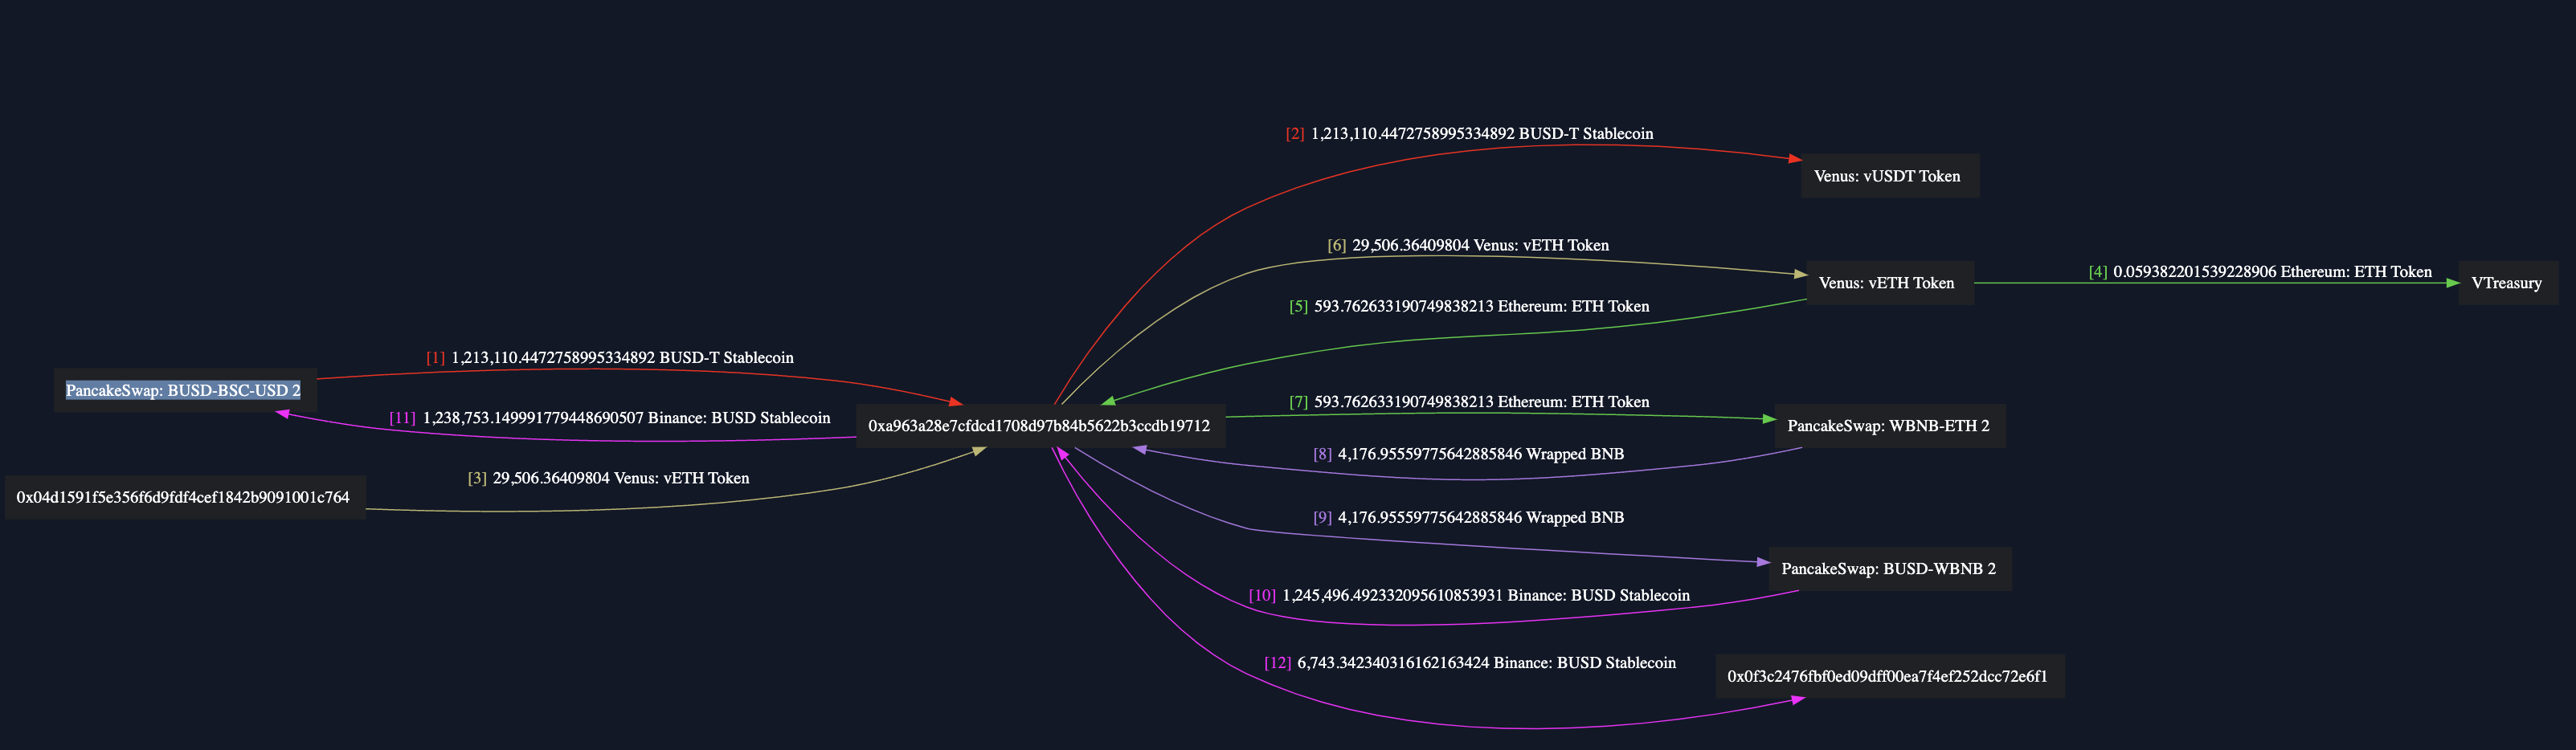
\includegraphics[scale=0.3]{img/liquidation_example.png}
  \caption{Tranzakcijos valiutų pavedimai \cite{liqpvz}}
  \label{img:liquidation_example}
\end{figure}

\begin{enumerate}
  \item \textbf{Trumpalaikė paskola.}  
  (1) pavedimu likvidatorius iš valiutų keityklos gauna 1213110 BUSD-T, su sąlyga, kad toje pačioje transakcijoje grąžins kitą valiutą – BUSD. Tai yra pirmasis žingsnis akimirksnio apsikeitimo (angl. \textit{flash swap}).

  \item \textbf{Likvidacijos veiksmai.}  
  (2) ir (3) pavedimais likvidatorius persiunčią visą prieš tai gautą BUSD-T į vUSDT baseiną, taip dalinai grąžindamas 0x04d... skolininko skolą. Mainais iš skolininko sąskaitos gauna vETH (\textit{Venus} protokolo apgaubtas ETH).

  \item \textbf{vETH konvertavimas į įprastą ETH.}  
  (5) ir (6) pavedimais likvidatorius išsikeičia turimus vETH į paprastą ETH, iš viso gaudamas 593,76 ETH.

  \item \textbf{ETH konvertavimas į BUSD.}  
  (7)--(10) pavedimais likvidatorius keičia ETH į BUSD tam, kad galėtų grąžinti trumpalaikę paskolą pirmajai keityklai. Po dviejų keitimų gauta 1245496 BUSD.

  \item \textbf{Skolos grąžinimas keityklai.}  
  Kadangi BUSD-T buvo gautas pirmajame pavedime, (11) pavedimu 
  grąžina 1238753 BUSD (maždaug 99,45\% iš (10) gautos sumos) pirmajai keityklai.

  % \item \textbf{Pelnas likvidatoriui.}  
  % Po visų veiksmų likvidatoriaus piniginėje lieka 6743 BUSD, kurie (12-uoju pavedimu) pervedami į pelno piniginę. BUSD prilygsta JAV dolerį, todėl galutinės pajamos \$6743, kur mokestis už tranzakciją \$204, todėl pelnas \$6539.

  \item \textbf{Pelnas likvidatoriui.}  
Po visų veiksmų likvidatoriaus piniginėje lieka 6743 BUSD, kurie (12-uoju pavedimu) pervedami į pelno piniginę.  
Kadangi BUSD prilygsta JAV doleriui, galutinės pajamos yra 6743 JAV doleriai.  
Sumokėjus 204 JAV dolerių tranzakcijos mokestį, likvidatoriui lieka 6539 JAV dolerių pelnas.
\end{enumerate}

\noindent
Jeigu likvidatoriui nereikėtų mokėti valiutų konvertavimo mokesčių, 
jam užtektų grąžinti apie 90,91\% (likvidacija grąžina 110\% įdėtos vertės) 
gauto užstato po likvidacijos. Tačiau realybėje egzistuoja tiek 
konvertavimo mokesčiai, tiek rinkos kainos gali skirtis nuo orakulo 
duomenų, todėl likvidatoriui teko grąžinti apie 99,45\% galutinės 
gautos valiutos.

\subsubsection{Atkartojimas}

\begin{table}[h!]
  \centering
  \begin{tabular}{|l|l|}
    \hline
    Mokestis už vieną kuro vienetą                           & 0,000000316441261625 BNB        \\
  \hline
  \multicolumn{2}{|c|}{\textbf{Likvidacija}}                              \\ \hline
  Grąžinta suma                            & 1213110,4472758995334892 BUSD-T         \\ \hline
  Užstato gauta \textit{wrapped} formatu             & 29506,36409804 vETH                     \\ \hline
  Kuro sunaudota dėl grąžinamos sumos patvirtinimo            & 24263                              \\ \hline
  Kuro sunaudota likvidacijos iškvietimui              & 816562                             \\ \hline
  Grąžinamos valiutos kaina               & 1,00148308 \$/BUSD-T               \\ \hline
  Užstato valiutos kaina          & 2250,50651698 \$/ETH            \\ \hline
  \multicolumn{2}{|c|}{\textbf{Užstato išsigryninimas (\textit{redeem})}}                                         \\ \hline
  \textit{Gas} sunaudota išsigryninimui                   & 141054                             \\ \hline
  Užstato gauta           & 593,762633190749838213 ETH             \\ \hline
  BNB kaina                & 298,22744081 \$/BNB             \\ \hline
  Pajamos                & \$121357,088416942287              \\ \hline
  Pelnas                 & \$121264,427054685937748              \\ \hline
  \end{tabular}
  \caption{Reikšmės atkartojus likvidaciją}
  \label{liquidation_example_repeat}
  \end{table}

\ref{liquidation_example_repeat} lentelėje pateikti skaičiai gauti pakartojus likvidaciją. Matome, kad pajamos yra 121 tūkstantis, kur \ref{img:liquidation_example} pav. pajamos yra tiktais 6,7 tūkstančiai. Šis skirtumas atsiranda iš to, kad orakulo kaina nesutampa su tuo ką gavo likvidatorius atliekant konvertavimus. Paimkime net pirmą konvertavimą po likvidacijos - ETH į BNB. Pakal orakulo kainas likvidatorius turėjo gauti 4480,7 BNB, tačiau gavo 4176,95 (6,78\% mažiau). Tai gali būti tiek dėl orakulo ETH pervertinimo, o gal ETH-BNB keitykla tuo metu turėjo prastą kainą ir/arba mažą likvidumą. Pažymime, kad mūsų tyrimui šis skirtumas nėra svarbus, nes koncentruojamės tik į likvidacijos dalies optimizaciją ir proporciškai lyginame gautą užstatą.

\subsubsection{Strategijų lyginimas}

Toliau lyginame skirtingas strategijas. Iš \ref{liquidation_example_comp} lentelės duomenų matome, jog originali likvidacija (\$1,21M) buvo kur kas mažesnė nei kokia galėjo ji būti (\$75,49M) su strategija \textit{iki uždarymo ribos}. Imant tiesiog orakulo valiutų vertes buvo galima pelnyti \$7,54M, tačiau tai reikalautų valiutų konvertavimų dideliais kiekiais. Prekiaujant tokias sumas reikėtų labai likvidžių rinkų ir galimai reikėtų skaidyti konvertavimus per kelias rinkas, kad išvengti didelių kainų svyravimų. Originalus likvidatorius jau su \$1,21M vertės konvertavimais patyrė nepalankias kainas. Apie kitų rinkų likvidumą pakomentuoti negalime, nes tai reikalautų papildomos istorinės tų metinių rinkų analizės.

Vis dėlto, buvo galima likviduoti dar didesnį kiekį nei \$75,49M pasinaudojus pasiūlyta \textit{pilno išeikvojimo} strategija. \ref{liquidation_example_comp} lentelėje šiai strategijai yra bendroji eilutė ir papildomai išskaidytos dvi dalinės likvidacijos. Pirmosios likvidacijos dydis \$36,27M ir po jos skolininko pozicijos sveikumo koeficientas turėtų būti truputi didesnis nei 1. Antrosios likvidacijos dydis \$46,24M vertės, tai reiškia, kad iš viso buvo grąžinta \$82,56M skolos, todėl ir atlygis už tai proporcingai didesnis. Atidžiai žiūrint į mokestį už kurą, galima pastebėti, kad 2 likvidacijų kuro suma lygi 1465384, tai yra mažiau nurodyto 1630707 prie bendros eilutės. Į bendrą yra papildomai pridėtas \textit{Venus} apgaubtos užstato valiutos konvertavimas, kurio užtenka iškviesti vieną kartą, pirmiausia atlikus abi likvidacijas, nes likvidacijos užstatas atsiimamas apgaubtu formatu.

\begin{table}[h!]
  \centering
  \begin{tabular}{|l|c|c|c|c|}
  \hline
  \textbf{Strategija}                & \textbf{Grąžinimas}    & \textbf{Paimtas užstatas}   & \textbf{Mokestis už kurą}            & \textbf{Pelnas}              \\ \hline
  Atkartoti                         & 1,21M (\$1,21M)         & 594 (\$1,34M)                & 981 879 (\$92,66)            & \$121,26K                    \\ \hline
  Iki uždarymo ribos                   & 75,37M (\$75,49M)       & 36,89K (\$83,03M)            & 981 888 (\$92,66)            & \$7,54M                      \\ \hline
  \makecell[cl]{Pilnas išeikvojimas \\ (bendras)}                   & 82,44M (\$82,56M)       & 40,35K (\$90,81M)            & 1 630 707 (\$153,89)         & \$8,25M                      \\ \hline
  \makecell[cl]{Pilnas išeikvojimas \\ (1 likvidacija)}                         & 36,22M (\$36,27M)       & 17,73K (\$39,89M)            & 816 591 (\$77,06)            & \$3,99M                      \\ \hline
  \makecell[cl]{Pilnas išeikvojimas \\ (2 likvidacija)}                        & 46,23M (\$46,24M)       & 22,63K (\$50,92M)            & 648 793 (\$61,23)            & \$4,26M                      \\ \hline
  \end{tabular}
  \caption{Skirtingų likvidavimo strategijų rezultatai}
  \label{liquidation_example_comp}
  \end{table}

\subsection{Strategijų vertinimas remiantis dideliais duomenų rinkiniais}
\label{sec:lyginimas_daug}

Skirtingoms strategijoms lyginti patogu naudoti kaupiamojo pelno kreivę. Galime analizuoti kiekvieną įvykusią likvidaciją, apskaičiuoti pelną pagal skirtingas strategijas ir laikui bėgant sumuoti pelnus. Tačiau, kaip matome iš \ref{liquidation_example_comp} lentelės, istorijoje ne visi likvidatoriai maksimaliai išnaudojo leidžiamą likvidacijų potencialą, o didelės galimybės dažnai yra suskaidomos į daug mažesnių likvidacijų. Dėl šios priežasties būtų klaidinga sumuoti pelnus kiekvienai įvykusiai likvidacijai, nes pelnai pagal geresnes strategijas būtų skaičiuojami kelis kartus. Problema kyla iš to, kad likvidacija turi įtakos kitoms su ja susijusioms likvidacijoms ir joms gali pakenkti jeigu pamodifikuotume ankstesnę likvidaciją. Dažniausias ryšys tarp skirtingų likvidacijų – tas pats skolininkas. Kiti galimi susiejimai: viena likvidacija išnaudoja visą likusį grynųjų likutį iš \textit{Venus} valiutos baseino, todėl kiti likvidatoriai netenka galimybės gauti grynųjų; likvidatoriai išnaudoja rinkos likvidumą keisdami valiutas.

Norėdami ir tokioje situacijoje pavaizduoti kaupiamąją pelno kreivę, laikysimės kelių apribojimų: analizuosime tik vieną kiekvieno skolininko likvidaciją istorijoje, pasirinkdami pirmąją, kurios metu buvo galima visiškai išgryninti visą gautą užstatą visomis trimis strategijomis. Laikantis šių apribojimų gauname 10892 įvykių iš 63982 analizuojamų (17,02\%). Taigi atlikę kiekvienai istorinei likvidacijai analizę kaip \ref{liquidation_example_comp} lentelėje ir susumavę pelną per laiką (kas atitinka ėjimą per blokus) gauname rezultatą \ref{img:bendras2} pav.

\begin{figure}[H]
  \centering
  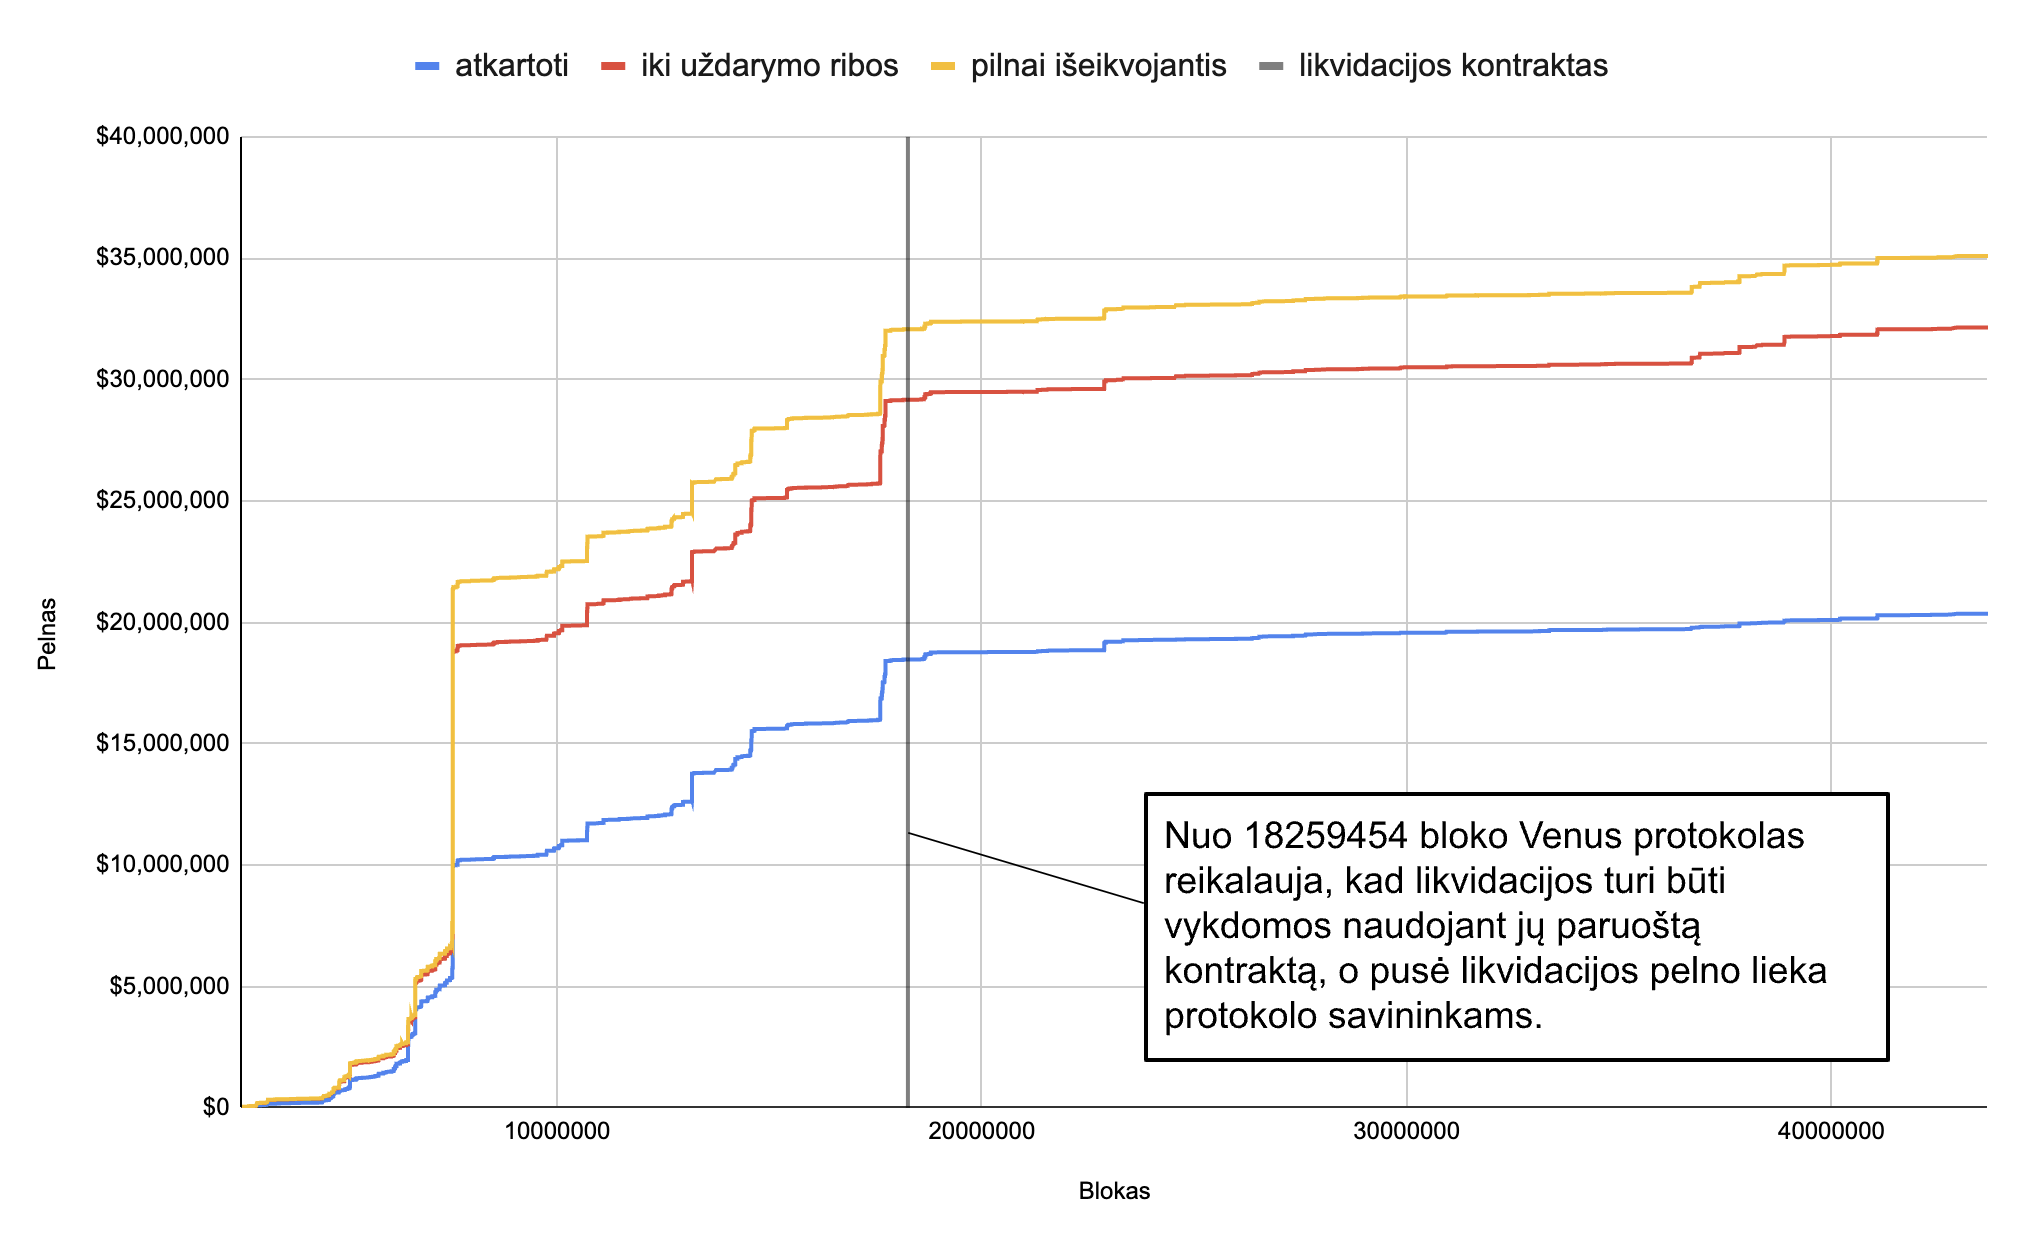
\includegraphics[scale=0.4]{img/bendras4.png}
  \caption{Kaupiamasis pelnas pagal strategijas, atsižvelgiant tik į pirmąją kiekvieno skolininko likvidaciją}
  \label{img:bendras2}
\end{figure}

\begin{table}[h!]
  \centering
  \caption{Strategijų pelnai}
  \label{tab:strategiju_pelnai}
  \begin{tabular}{|l|r|}
  \hline
  \textbf{Strategija}                     & \textbf{Pelnas (\$)} \\ \hline
  Atkartoti                               & 20 355 860,62        \\ \hline
  Iki uždarymo ribos              & 32 149 135,99        \\ \hline
  Pilnas išeikvojimas                           & 35 089 532,28        \\ \hline
  \end{tabular}
  \end{table}

Rezultatai \ref{tab:strategiju_pelnai} lentelėje rodo, kad laikantis nurodytų ribojimų \textit{iki uždarymo ribos} strategija generavo 58\% didesnį pelną nei \textit{atkartoti}, o \textit{pilnas išeikvojimas} strategija – net 72\% daugiau. Pastebėtina, kad reikšminga dalis prarasto pelno yra susijusi su tuo, jog likvidatoriai dažnai negrąžina maksimalios leistinos sumos. Be to, yra maždaug 9\% potencialas padidinti pelną naudojant efektyvesnį likvidacijos algoritmą.

Galime atkreipti dėmesį, kad \ref{img:bendras2} pav. visų strategijų pelno kreivės yra panašios, jei atmesime kelis išskirtinius staigius šuolius tam tikruose laiko momentuose. Tai reiškia, kad strategijų pelno skirtumą smarkiai veikia keletas įvykių.

Nuo 18259454 \cite{LikvidacijosKontraktas} bloko \textit{Venus} protokolas pakeitė likvidavimo mechanizmą. Po pakeitimo visos likvidacijos privalo būti vykdomos per \textit{Venus} protokolo parengtą kontraktą, kuris pasilieka pusę likvidacijos pelno, 5\% nuo likviduojamos sumos, ir kitus 5\% atiduoda likvidatoriui. Po šio pakeitimo pastebimas reikšmingas pelno lėtėjimas, tačiau tai taip pat gali būti susiję su tuo, kad laikui bėgant į grafiką patenka vis mažiau likvidacijų, nes analizuojame tik po vieną likvidaciją vienam skolininkui.

\subsubsection{Išskirtiniai atvejai}

Blokų ruože 7544850–7546511 įvyko trys didelės likvidacijos, kurių metu pastebėtas reikšmingas skirtumas tarp strategijų:

\begin{enumerate}[label=\textbf{\Alph*.}]
    \item 0x0cd0fc0cdd5b572d71cd039cc522d20dfcc5c8c0772173b484c91194401fe89b – blokas 7544850
    \item 0x718cf2813f3124f576a64a69429ec543ea6b14ca53d557772d61e72a6c256f3e – blokas 7546281
    \item 0x3b04a03ed356108c7297e6b438d70df7383f10d39d0511603b576b635d6bff9f – blokas 7546511
\end{enumerate}

\begin{table}[h!]
  \centering
  \caption{Strategijų pelno palyginimas (skliaustuose likvidacijų iškvietimų skaičius)}
  \label{tab:profit_table}
  \begin{tabular}{|l|c|c|c|}
  \hline
  \textbf{Strategija}        & \textbf{A}          & \textbf{B}          & \textbf{C}          \\ \hline
  Atkartoti                  & \$2 015 683      & \$190 227       & \$15 074        \\ \hline
  Iki uždarymo ribos         & \$2 015 683      & \$6 630 951      & \$1 060 317      \\ \hline
  Pilnas išeikvojimas        & \$4 031 270 (50)      & \$6 630 951 (1)      & \$1 083 910 (2)      \\ \hline
  \end{tabular}
  \end{table}

Įdomu yra tai, kad visi trys nagrinėjami atvejai išsiskiria savo duomenimis dėl skirtingų priežasčių:

\begin{enumerate}[label=\textbf{\Alph*.}]
  \item Pirmuoju atveju originalioje tranzakcijoje likvidatorius grąžino maksimalią leistiną sumą per vieną likvidacijos funkcijos iškvietimą. Dėl šios priežasties \textit{atkartoti} ir \textit{iki uždarymo ribos} strategijų pelnai buvo identiški. Šiame scenarijuje skolininkas buvo reikšmingai įsiskolinęs, todėl likvidavimo procesas galėjo būti tęsiamas net 49 kartus, kiekvieną kartą grąžinant dvigubai mažesnę sumą nei ankstesnėje iteracijoje. Galutinis pelnas, pasiektas vykdant šį procesą, buvo beveik du kartus didesnis už \textit{iki uždarymo ribos} strategijos pelną.

  \item Antruoju atveju likvidatorius pasirinko likviduoti žymiai mažesnę sumą, nei leido protokolo uždarymo riba. Dėl to \textit{iki uždarymo ribos} strategijos pelnas buvo maždaug 35 kartus didesnis nei \textit{atkartoti} strategijos. Šiame kontekste likvidatorių ribojo ne uždarymo riba, o skolininko turimo užstato kiekis. Todėl \textit{Pilnas išeikvojimas} strategija šioje situacijoje reikalavo tik vieno likvidacijos iškvietimo, kad būtų maksimaliai išnaudota galimybė.

  \item Trečiuoju atveju, kaip ir antrajame, originalus likvidatorius grąžino mažesnę sumą nei leido protokolo nustatyta uždarymo riba. Tačiau šiuo atveju likvidatorių ribojo būtent uždarymo riba. Siekiant optimizuoti pelną, buvo atliktos dvi atskiros likvidacijos, kurios leido papildomai sugeneruoti \$23593 virš \textit{iki uždarymo ribos} strategijos pelno.
\end{enumerate}

\subsubsection{Atmestos likvidacijos}

Atkartojimo strategija pasirodė esanti veiksminga, nes buvo pastebėta, kad ne visas likvidacijas pavyktų atkartoti bet kuriam likvidatoriui. Analizės metu buvo atmestos likvidacijos, kurios turėjo privilegijuotą statusą ir galimybę jas vykdyti turėjo tik tam tikri adresai, galėję iškviesti likvidavimo funkciją:

\begin{enumerate}
    \item Likvidacijos, kurios toje pačioje tranzakcijoje atliko platformos konfigūracijos pakeitimus, leidžiančius likviduoti tam tikrus skolininkus:
    \begin{itemize}
        \item \texttt{0x7c97317afe5911e704bd684e8b3fe472d7b8703b54321ab564be2bbeacdb0f5f} – VIP-36 Refactor SXP \& XVS Collateral Factor and Interest Rate Model Change
        \item \texttt{0xc81fa724698490d096b04cccb080195517f4df5cfa56121cbee895d05ad0de53} – VIP-37 Refactor SXP \& XVS Collateral Factor and Reward Speed
        \item \texttt{0xb18543cd79c90ef2ca1e463aaf3760e6e4e731b7fa64a86e6f2538de392d49df} – VIP-223 Risk Parameters Adjustments (BUSD)
    \end{itemize}
    \item \textit{BNB bridge exploiter} likvidacijos, kur tik platformos savininkai sau leido likviduoti:
    \begin{itemize}
        \item Skolininko adresas: \texttt{0x489a8756c18c0b8b24ec2a2b9ff3d4d447f79bec}
        \item Viena iš 14 likvidacijų - \\0xc4bd0beaedfa6985c7976d6c1dd681ec1e4fa805067572e95beae32869c88cd7
    \end{itemize}
\end{enumerate}

Taip pat, nebuvo analizuojamos likvidacijos, kurios išnaudojo \textit{Venus} protokolo mechanizmo klaidą, susijusią su paskatų kaupimu naudojantis protokolu. Naudotojai, skolindami arba skolindamiesi protokole, kaupė atlygį, kurį galėjo atsiimti iškviesdami funkciją \textbf{claimVenus}. Įdomu tai, kad šią funkciją galėjo iškviesti bet kuris adresas kito naudotojo vardu. Tai suteikė galimybę išnaudotojams aptikti adresus, kurie buvo stipriai įsiskolinę ir sukaupę nemažą atlygį, atsiimti sukauptą atlygį jų vardu ir tuoj pat inicijuoti jų likvidaciją. Vienas tokio išnaudojimo pavyzdys užfiksuotas tranzakcijoje: 0x801001726f7c0c2434a8ea1680213ebfd5201094087c94d7dac44b7860555f1c. Šis pažeidžiamumas vėliau buvo pašalintas, įdiegiant apribojimą, kad \textit{claimVenus} funkcija negali būti sėkmingai iškviečiama, jei paskyros sveikatingumo rodiklis yra neigiamas \cite{exploitFix}.

\sectionnonum{Rezultatai ir išvados}

Šiame darbe analizuojama ir nagrinėjama likvidacijos kompleksiškumo problematika. Siekiant ją spręsti, iškeliamas tikslas, o šiam tikslui įgyvendinti pasiūloma esamo algoritmo modifikacija, siekiant didesnio pelno iš likvidatoriaus perspektyvos.

Darbe pristatomas egzistuojantis likvidavimo algoritmas – \textit{Optimal Fixed Spread Liquidation Strategy}. Taip pat siūloma ir nagrinėjama jo modifikuota versija, pavadinta \textit{pilno išeikvojimo} strategija. Modifikacijos pritaikytos \textit{Venus} paskolų platformai, kuri pasižymi specifinėmis ypatybėmis (pavyzdžiui, apgaubtų valiutų elgsenos niuansais). Be to \textit{pilno išeikvojimo} strategija yra pranašesnė tuo, kad efektyviai išnaudoja galimybes, kai skolininkas yra stipriai įsiskolinęs, ir taip pat optimizuoja likvidacijos procesą, kai likvidatorius yra ribojamas skolininko užstato kiekiu.

Surinkus duomenis nuo 2020-11-26 iki 2024-11-03, \textit{Venus} platformoje buvo palygintos trys likvidavimo strategijos: \textit{atkartoti}, \textit{iki uždarymo ribos} ir \textit{pilnas išeikvojimas}. Istoriniai duomenys atskleidė, kad ne visi likvidatoriai maksimaliai išnaudojo leidžiamą likvidacijos potencialą. \textit{Iki uždarymo ribos} strategija, nors ir paprasta, generavo 58\% didesnį pelną lyginant su istorinių likvidacijų rezultatais (atsižvelgiant tik į \ref{sec:lyginimas_daug} skyriuje lygintas likvidacijas). Pastebėta, kad \textit{pilnas išeikvojimas}, nors ir reikalauja daugiau likvidacijos iškvietimų, gali dar labiau padidinti pelną, ypač tais atvejais, kai skolininko įsiskolinimas yra didelis ir jį galima likviduoti pakartotinai. Naudojant \textit{pilną išeikvojimą}, galima gauti maždaug 9\% daugiau pelno nei taikant strategiją \textit{iki uždarymo ribos}, o iš viso net iki 72\% daugiau, jei likvidavimo procesas parenkamas optimaliai. Tačiau svarbu pabrėžti, kad reikšminga dalis papildomo pelno atsiranda iš palyginti nedidelio skaičiaus įvykių, kurie gali būti atsitiktiniai ir nebūtinai reprezentatyvūs būsimoms likvidacijoms ar kitoms istorinėms likvidacijoms kituose paskolų protokoluose bei/arba \textit{blockchain} tinkluose.

Ateityje planuojama tęsti šį darbą eksperimentuojant su užstato ir skolos grąžinimo valiutų pakeitimu į kitas. Pavyzdžiui, jeigu yra galimybe pasirinkti užstato valiutą su mažesniu likvidacimo slenkščiu, būtų mažiau paveiktas skolininko sveikumo koeficientas, o tai leistų likviduoti daugiau turto.

\printbibliography[heading=bibintoc] % Literatūros šaltiniai aprašomi
% bibliografija.bib faile. Šaltinių sąraše nurodoma panaudota literatūra,
% kitokie šaltiniai. Abėcėlės tvarka išdėstoma tik darbe panaudotų (cituotų,
% perfrazuotų ar bent paminėtų) mokslo leidinių, kitokių publikacijų
% bibliografiniai aprašai (šiuo punktu pasirūpina LaTeX). Aprašai pateikiami
% netransliteruoti.

% \appendix  % Priedai
% Prieduose gali būti pateikiama pagalbinė, ypač darbo autoriaus savarankiškai
% parengta, medžiaga. Savarankiški priedai gali būti pateikiami kompiuterio
% diskelyje ar kompaktiniame diske. Priedai taip pat vadinami ir numeruojami.
% Tekstas su priedais siejamas nuorodomis (pvz.: \ref{img:mlp}).

\end{document}